\documentclass[10pt,draftclsnofoot,onecolumn]{IEEEtran}
\hyphenation{op-tical net-works semi-conduc-tor}

\usepackage[margin=.75in]{geometry}
\usepackage{courier}
\usepackage{ifthen}
\usepackage{setspace}
\usepackage{listings}
\usepackage[usenames, dvipsnames]{color}
\usepackage{tabularx}
\usepackage[strict]{chngpage}
\usepackage{cite}
\usepackage{graphicx}
\usepackage{acronym}
\usepackage{color}
\usepackage{makeidx}
\usepackage{url}
\usepackage{listings}
\usepackage{verbatim}

\makeindex

\acrodef{NPM}[NPM]{Node Package Manager}
\acrodef{OSU}[OSU]{Oregon State University}
\acrodef{AIAA}[AIAA]{American Institute of Aeronautics and Astronautics}
\acrodef{COCOM}[COCOM]{Coordinating Committee for Multilateral Export Controls}
\acrodef{AGL}[AGL]{Above Ground Level}

\lstset {
	language=C,
	basicstyle=\ttfamily,
	keywordstyle=\color{blue}\ttfamily,
	stringstyle=\color{red}\ttfamily,
	commentstyle=\color{OliveGreen}\ttfamily,
	morecomment=[l][\color{magenta}]{\#}
	showstringspaces=false,
	showspaces=false,
	frame=single,
	captionpos=b
}

\newcommand{\commandline}[2][\empty] {
	\begin{quote}
		\texttt{#2}
		\ifthenelse{\equal{#1}{\empty}}{}{\begin{quote}#1\end{quote}}
	\end{quote}
}

\newcommand{\sigline}[1][\empty] {
	\vspace{1in}
	\hrule width0.5\textwidth
	\vspace{1mm}
	\noindent #1	
}

\newcommand*{\SignatureAndDate}[1]{
	\vspace{1in}
	\par\noindent\makebox[2.5in]{\hrulefill} \hspace{.5in} \makebox[2.0in]{\hrulefill}
	\par\noindent\makebox[2.5in][l]{#1}      \hspace{.5in} \makebox[2.0in][l]{Date}
}


\begin{document}
	\singlespace
	
	\title{\vspace{2in}Design}
	
	\author {
		Anisimova, Natasha
		\and
		Lee, Terrance
		\and
		Morgan, Albert
	}
	
	\markboth{CS Capstone 2016-2017}{Groundstation}
	
	\pagestyle{empty}
	\vspace*{2in}
	\begin{center}
		\huge
		Groundstation: Progress\\
		\normalsize
		\vspace{5mm}
		\textbf{
			Team \#25\\
			High-Altitude Rocketry Challenge\\
		}
		\vspace{1mm}
		Natasha Anisimova\\
		Terrance Lee\\
		Albert Morgan
	\end{center}
	
	\vspace{5mm}
	
	\begin{center}
		\textbf{Abstract}
	\end{center}
	
	%\begin{adjustwidth}{0.75in}{0.75in}
	
	%Abstract goes here
	The \textit{Groundstation} software will collect telemetry from a rocket while it is in flight and graphically display the telemetry in real-time. Groundstation is made up several different components: collection of data, storage of data, interpolation of data, and 
	display of data.
	This document will describe the progress that was made by the Groundstation software team over the course between September and December of 2016.
	%\end{adjustwidth}
		
	\pagestyle{headings}
	
	\newpage

	% Uncomment this to make the table of contents	
	\tableofcontents
	\newpage

\section{Purpose and Goals}
	In June 2017, the \ac{OSU} chapter of the
	\ac{AIAA} will launch a rocket at Spaceport America.
	This rocket will ascend to one hundred thousand feet \ac{AGL}.
	Designing, building, and launching the rocket will require the
	collaboration and expertise of dozens of engineers from a variety
	of disciplines, including mechanical, electrical, computer, and
	software.
	
	Many rockets record data during the flight. This data may include
	altitude, latitude, longitude, and more.
	Latitude and longitude
	data is helpful for locating the rocket after it lands, but
	if the data is located on the rocket, then it is useless
	for this task.
	Altitude data will tell the rocketry team if we have
	met the objective of one hundred thousand feet, but if the rocket
	is damaged or cannot be located for any reason, then the record
	of this achievement may be lost.
	
	However, the chicken-and-egg problem of not being able to access
	the location data before the rocket is found may be avoided by sending
	telemetry from the rocket in real-time.
	Telemetry may be received wirelessly
	by the rocketry team while the rocket is in flight, giving them
	access to useful information such as the rocket's last known location
	and the highest altitude reached. This telemetry will aid in the
	rocket's recovery and provide a log of the rocket's flight even if
	recovery is impossible.

\section{Current Progress}
All our requirements our done.  Albert completed the Web Server, Web Backend and Logging of Data. He also was helping some of the avionics team with some coding with their physical groundstation and did a lot of integration to work out bugs with them.  Natasha completed the Data Visualization, User Interface Organzation, User Interface Interaction Model.  We have a beautiful 3D visualization and a very well organized website that can our team can locate what pieces of data that want during the launch without hassle.  Terrance completed his Retrieval, Interaction Model, and Toolkit to Generate the User Interface (UI).  We have a smooth way of retrieving the data so that we are able send it to our visualizations to be used.  Figure 1 shows the 3D representation of the rocket launching from Spaceport America.

\section{The Future}
We have one more test launch in Brothers, OR on May 20. This launch will be our final integration test with the whole team. After that we will make any minor adjustments and make any preparations for our presentation launch at Space Port America in New Mexico. Terrance will have to redo the Retrieval requirement in more detail in the final progress report video.  This is due to the Electrical Engineering team having their radios go bad on them when we last went out to Brothers.  Hopefully this will be fixed during our next test launch. 

\begin{figure}[h]
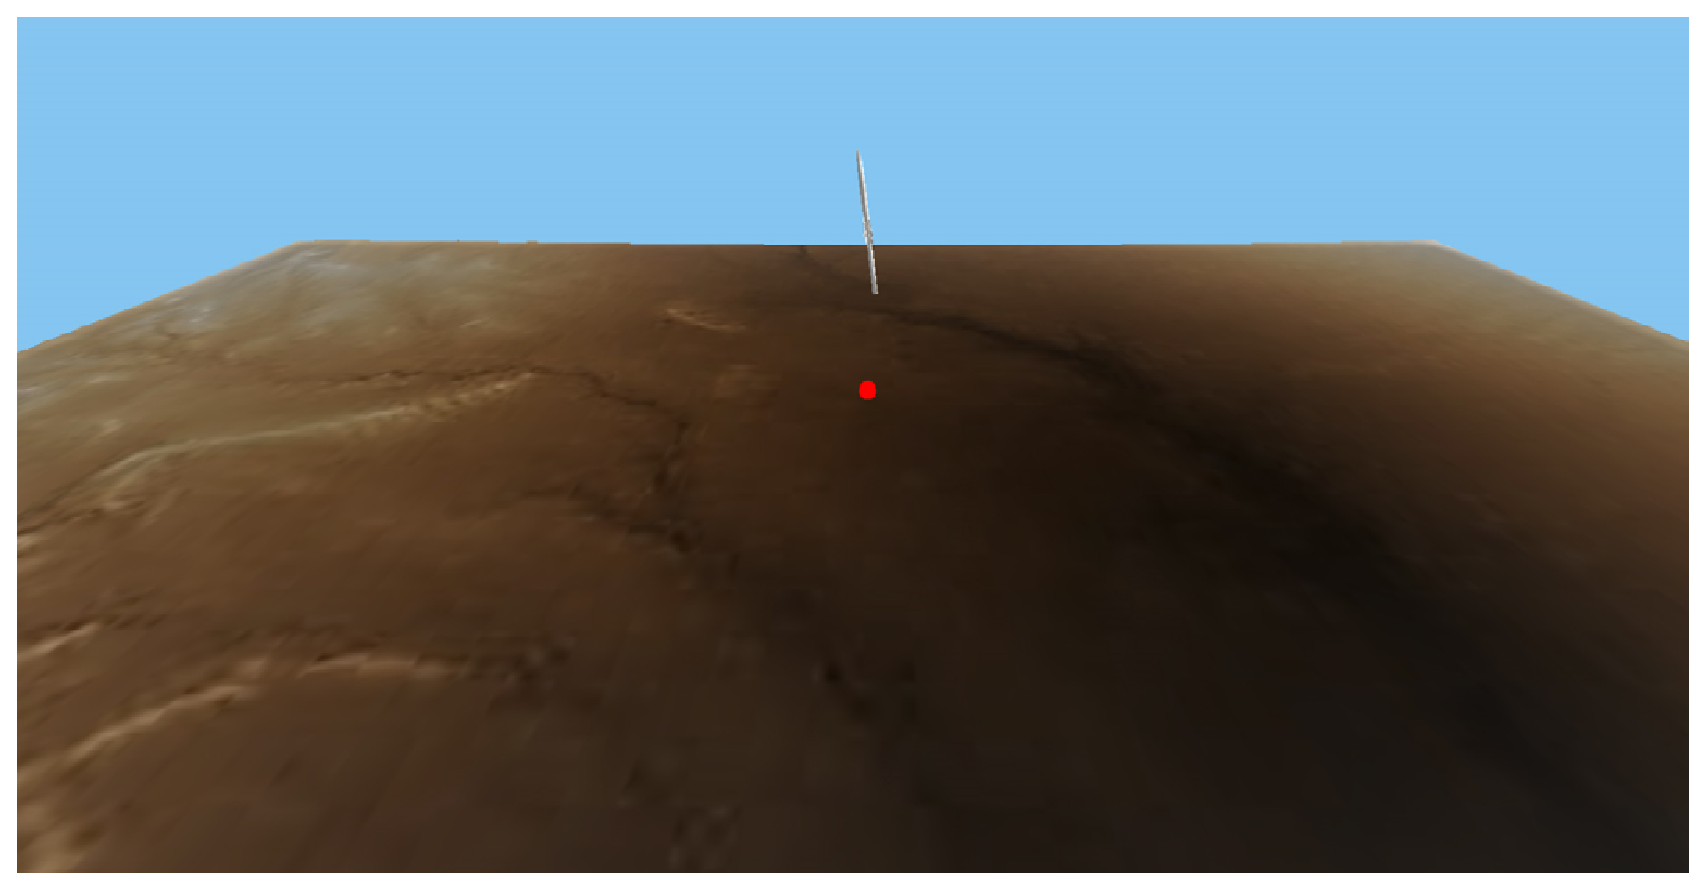
\includegraphics[width=6in]{flight}
\caption{The 3D view of the rocket launch.}
\end{figure}


\section{Development Log}


\subsection{Week 1}
\subsubsection{Anisimova, Natasha}
\begin{itemize}
	\item \textbf{Plans: }
	For this next week I need to figure out the scale and load the terrain into the webpage. Colorizing it would be good as well. The Avionics and Recovery Team want to do an integration test soon as well so we need to keep that in mind. 
	\item \textbf{Progress: }
	Now that we have the height map and Al was able to get an image out of the .xtr file, I was able to get a 3D model of the 	terrain around Spaceport America. Scaling is now our biggest concern. 
	\item \textbf{Problems: }
	Figuring out the longitude and latitude scale compared to miles for the model. It seems like the 3D model is skewed a bit. The east and west were elongated slightly. The webpage needs to be re-organized as well. Having the 3D terrain be the first thing that a person sees would be ideal. 
\end{itemize}

\subsection{Week 1}
\subsubsection{Lee, Terrance}
\begin{itemize}
	\item \textbf{Plans: }
	I have a meeting with Ben Brewster who knows more about networking next week. I want to get systemd implemented into inittab. Get the layout for the line graph layout at minimum if not more so that we can get that setup. Also want to get our final link setup or at least a link setup that we can use for expo so that I have a network that I can use for the line graph setup. 
	\item \textbf{Progress: }
	I found a good resource for our Live Line Graph for the rocket and I found what was need for Systemd and inittab to work together. I also went to a meeting with avionics and recovery about a couple of things that they wanted to get covered and make sure everybody was on the right page. We were originally not needed for this meeting but I am glad I went but cause there was a few things that we should know about and somethings that we might want to talk about as well in our next meeting that we may want to put into our code. 
	\item \textbf{Problems: }
	Having a issue with line graph that I am using. I can hook it up to a network but it used to using websites but since we are using a raspberry pi as our network I have to ask others who know more about networking for help on this. This is why I have a meeting with Ben Brewster next week. 
\end{itemize}


\subsection{Week 1}
\subsubsection{Morgan, Al}
\begin{itemize}
	\item \textbf{Plans: } 
	Over the course of the next week I hope to finish the 3D interface and get it into something resembling its final form. Additionally, the avionics team is ready for integration testing, so I will ensure that our software is ready to interact with their hardware. the protocol has changed since we began to the project, so a few minor changes will need to be made before the software is ready to integrate, but since the framework of the protocol is already in place I do not believe that this will cause any major issues. 
	\item \textbf{Progress: }
	This week we began integrating the 3D model into the web interface. We took the new, higher resolution height map data and turned it into an image, which we then used to construct a 3D model (a .obj file) that we can import into the WebGL canvas using Three.js. I also got some very basic objects to move around the scene to represent the rocket. I haven't actually hooked the moving objects into the telemetry data yet, but all of the pieces are in place to do so. 
	\item \textbf{Problems: }
	We had a minor hiccup when we realized that the Earth is round and one degree of latitude does not equal one degree of longitude in terms of distance. However, some quick and easy trigonometry fixed this issue.
\end{itemize}

\subsection{Week 2}
\subsubsection{Anisimova, Natasha}
\begin{itemize}
	\item \textbf{Plans: }Getting the atmospheres to be at the correct height will be a problem since everything has to be scaled correctly according to the data that we are receiving. The 3.js transparency works, we just need to make sure that we have all the correct libraries for it and that it is set up correctly in the environment. 
	\item \textbf{Progress:} Originally the terrain that I had created was off in terms of scale to longitude and latitude compared to Google Earth. Al was able to figure out the math behind it and alter it. The terrain also had a distorted height values due to how Blender was adding the modifier for height of the height map image to the flat plane. After speaking to the rest of the mechanical engineers, they said they wanted it to be as close to the realistic area as possible. This lead us to having a quite a flat plane. I have also been working on transparency since that will be useful for showing the different atmospheres that the rocket is going through. 
	\item \textbf{Problems: } 
	Telemetry protocol is changing. Hopefully this will be the last time.
	
	
\end{itemize}

\subsection{Week 2}
\subsubsection{Lee, Terrance}
\begin{itemize}
	\item \textbf{Plans: } 
	I want to have a dynamic graph built by the end of next week and we should be ready to integrate with the log that Al built for the expo.
	\item \textbf{Progress:  }
	This week I switched what type of live line graph I was going to use for our demo. The one I found was much simpler. I also spoke to my old network instructor Ben Brewster about how we should go about receiving the call from the sensor whether we would have to setup a network on the graph code or with the through the packet code itself. He explain both ways and suggested that on the website that we would use would need a simple ajax call and just build the graph in html with the javascript. I tested his idea with another dynamic javascript setup I had an it works.
	\item \textbf{Problems: }
	The only real problem I am having is finding enough time to be honest. I wanted to get the graph done by this weekend but I have so much homework that needs to be done first that is why I have to push it back to the end of this week. I should be able to get it done before then but I just don't want to say it will be done and it is not.
\end{itemize}


\subsection{Week 2}
\subsubsection{Morgan, Al}
\begin{itemize}
	\item \textbf{Plans: }
	This week I'm going to get the 3D model we made loaded into the web interface and ensure that it is scaled correctly by creating some test data that should map to the corners of the 3D model. We can then see whether or not the model is scaled correctly. Additionally, I will keep up with the avionics team to make sure that we are implementing the correct telemetry protocol.
	\item \textbf{Progress: }
	This week I got the 3D model of the terrain at the launch site properly scaled in all axes. The 3D model is very flat when rendered this way because the site is in the middle of the desert. However, we may be able to use some lighting tricks to make it more visually interesting.
	
	The telemetry protocol has been a moving target, so I ensured that we are implementing the most recent standard from the avionics team. However, the protocol is going to change again in the next week or two, so this work isn't finished.
	\item \textbf{Problems: }
	Getting the 3D model scaled took a little longer than I expected, and the telemetry protocol is changing again, so progress was a little slow this week, but there are no significant issues.
\end{itemize}

\subsection{Week 3}
\subsubsection{Anisimova, Natasha}
\begin{itemize}
	\item \textbf{Plans: }
	This weekend we are planning on meeting up with the Avionics team and integrate our work with theirs. I also hope to make the interface a little bit more intuitive, add some more controls and an actual rocket.
	\item \textbf{Progress:  }
	We reviewed our poster with Team 24 this week. We got a good idea of what they were doing and some constructive feedback for our own poster. Everything seems to be wrapping up. The website was split up into something that was more useful instead of being all on one page.
	\item \textbf{Problems: }
	I do not have the Arduino so I can only see the data being mocked when with the rest of the team. There is a problem with the table not updating when the user goes to a different part of the website. When the user goes back to the table it is empty. It just starts displaying data from the second that the user goes back to the table, none of the previous data.
\end{itemize}

\subsection{Week 3}
\subsubsection{Lee, Terrance}
\begin{itemize}
	\item \textbf{Plans: }
	We have integration with the electronic team on Saturday. Update our poster and have Dr. Squires to take a look at it. If she approves have the final sent in. Clean up any issues before the code freeze that is coming up. If I finish my part early help my anyone in my group so that we can all finish before the freeze.
	\item \textbf{Progress:  }
	I was able to finally get the 2D Dynamic line graph code I made working on a website that I made working. The time and altitude adjusts to real time of the data during the rocket flight. We also reviewed and had our poster reviewed of group 24 this week as well.
	\item \textbf{Problems: }
	The issue this week a simple script src issue. I was so busy with other homework this week that I missed this simple error.
\end{itemize}


\subsection{Week 3}
\subsubsection{Morgan, Al}
\begin{itemize}
	\item \textbf{Plans: }
	This weekend we are planning to met with the avionics team to do integration testing with their side of the system. There are also some more things to discuss about the final protocol. Later in the week, I hope to smooth the rough edges out of the frontend and get it looking really nice.
	\item \textbf{Progress: }
	This week we finally integrated the frontend and the backend. The web site will get data (currently being faked by an Arduino) and represent the position of the fake rocket on a 3D display showing the terrain of the launch site.
	\item \textbf{Problems: }
	The 3D components of the frontend took a little longer to get together than I anticipated, but no major problems.
\end{itemize}

\subsection{Week 4}
\subsubsection{Anisimova, Natasha}
\begin{itemize}
	\item \textbf{Plans: }
	This weekend there is going to be test launch in Brothers, Oregon. There is a possibility that the rocket will not be retrieved since this is the first time we are testing the recovery with an actual rocket. Luckily the team is prepared to make another board for the Avionics team if that happens.
	\item \textbf{Progress:  }
	The 3D visualization is now a part of web application. The website is now a lot cleaner and we have just been removing files that were used in previous versions or drafts of our project. Everything is coming together full circle and integration with the Avionics Team is hopefully complete.
	\item \textbf{Problems: }
	We had one problem with getting rid of an internet dependencies but after an email it was resolved. We now do not have to worry about creating the line graph that is updating from scratch.
\end{itemize}

\subsection{Week 4}
\subsubsection{Lee, Terrance}
\begin{itemize}
	\item \textbf{Plans: }
	Since I can't make it to brothers I am waiting until Monday to see what data we got back from test launch that we had at brothers. At this point I am going to work on anything that we need to get done for expo. If there is anything major help fix it. Anything minor help fix it. I am going to hold off on the parachute signal until after we have what we need for all our requirements done since that is a extra thing I am doing for the recovery team. Also implement the canvasjs correct platform that we received from them.
	\item \textbf{Progress:  }
	I cleanup the 2D line graph code and added it to the server. Al had added the logger to it so that it will now receive the altitude that it was made to receive instead of some random math generator that was made. I am working on the after expo part of it so that it can receive the parachute "signals" for the launch so that it is seen on the graph.
	\item \textbf{Problems: }
	No major Problems after we got the OK from the CanvasJS.com to use their website platform for free.
\end{itemize}


\subsection{Week 4}
\subsubsection{Morgan, Al}
\begin{itemize}
	\item \textbf{Plans: }
	This weekend we are doing a test launch. I am writing this as we are waiting to leave for Brothers, Oregon for the weekend. There, we will launch a rocket similar to the upper stage of our final rocket and ensure that the avionics is functional.
	\item \textbf{Progress: }
	I spent every day this week integrating our software with the avionics. There were some problems on our end as well as their end, but in the end we managed to get everything working together.
	\item \textbf{Problems: }
	Other than the time spent getting everything working with avionics, there were no problems this week.
\end{itemize}

\subsection{Week 5}
\subsubsection{Anisimova, Natasha}
\begin{itemize}
	\item \textbf{Plans: }This weekend is a huge test launch that most of the HART team will be attending. All the computer scientists in our sub team will be there. I am currently torn between working on the new requirements after code freeze or continuing on with the 3D visualization. Either way, work will continue. Lights and displays on the groundstation (the box full of hardware) is now being integrated.
	\item \textbf{Progress:  }
	We had a bunch of new requirements that came up out of nowhere. We designed our software to visual and present data, not send anything back the other way.
	\item \textbf{Problems: }
	Huge last-minute changes due to new requirements for locating the rocket. We will be controlling the launch button which requires taking security measures into account. We had designed our software to take lots of data in and be able to handle that in any way, not send data anywhere.
\end{itemize}

\subsection{Week 5}
\subsubsection{Lee, Terrance}
\begin{itemize}
	\item \textbf{Plans: }
	During this launch on Saturday we are launching our sustainer so I will be able to see how well the live line graph actually works at a higher and faster launch. Also with the new parachute changes that are being put in can be put in next week.
	\item \textbf{Progress:  }
	This week we got our poster approved. I personally did not get much work done this week because of midterms and preparing for the launch this weekend.
	\item \textbf{Problems: }
	My two midterms and my two quizzes. I had to study for all them took up so much time. I have to thank my great team for their support.
\end{itemize}


\subsection{Week 5}
\subsubsection{Morgan, Al}
\begin{itemize}
	\item \textbf{Plans: }
	We are leaving to Brothers this weekend for the second test launch. After the launch, I plan on continuing to work on the new groundstation control portion of the code. We have met all of our requirements, and were simply polishing our stretch goals at this point, so I plan on personally halting all work on those stretch goals and working with the avionics team to make sure they are ready for the final launch.
	\item \textbf{Progress: }
	This week we got hit by massive last-minute scope creep. The avionics team thought that we were writing software to control the groundstation this entire time, but didn't mention it to us until yesterday: the day before we left for our second and final test launch. We have been working furiously to try to get the groundstation ready for the real launch in June, but many of our initial design parameters may have to be compromised to meet these new requirements.
	\item \textbf{Problems: }
	The day before we left for our second test launch, the avionics team revealed to us that they were expecting us to control various aspects of the groundstation. For example, lights, LCD, and the launch button. This is an enormous last-minute change in requirements. We designed our software from the beginning to only collect data and to be extremely stable so that data isn't lost. However, if we are controlling the actual launch codes, our primary concern becomes safety, and the parameters of our entire software package changes. Our software was simply not designed with these concerns in mind, and adding them with one month to go after eight months of work may prove problematic.
\end{itemize}

\subsection{Week 6}
\subsubsection{Anisimova, Natasha}
\begin{itemize}
	\item \textbf{Plans: }
	We got the correct equation for converting the GPS minutes, seconds, into decimals. We now hope to successfully test launch as long as nothing else goes wrong with the power supply.
	\item \textbf{Progress:  }
	We went to Brothers, Oregon last week. Unfortunately we were unable to launch due to a number of reasons. Thankfully none of it had to do with errors with the software.
	\item \textbf{Problems: }
	There were a number of problems that happened with the Avionics Team, as well as weather. There were high winds earlier in the day and even snow. Later in the day the skies cleared though but the team found other errors. One thing I noticed was that the GPS longitude and latitude were being passed as minutes and seconds instead of decimal values like we were expecting.
\end{itemize}

\subsection{Week 6}
\subsubsection{Lee, Terrance}
\begin{itemize}
	\item \textbf{Plans: }
	This weekend and Monday if needed I plan on doing my part for the video for our midterm progress report and preparing for the expo.
	\item \textbf{Progress:  }
	Due to some errors with avionics last week we didn't get a launch at brothers. Our team overall made a final decision where the EE team of avionics will not control the parachutes or the separation of the two stages or the re-ignition of the sustainer. That will now be handled by the ME team of avionics. Since that is happening the live line wire graph plan of showing when those points where going to happen is closed now. The EE's will not be putting those sensors on the rocket anymore so we will not be getting that data back so I include that on that graph.
	\item \textbf{Problems: }
	I spoke with John our TA Friday morning about how our Mocker looked for the live line graph. He gave us some suggestions, I told him what I planned on doing and of course awesome AL just did it right there even before we even finished talking and just showed it to him to make him happy.
\end{itemize}


\subsection{Week 6}
\subsubsection{Morgan, Al}
\begin{itemize}
	\item \textbf{Plans: }
	There is likely to be another test launch next week, after expo. However, there isn't much left for us to do, so I plan on focusing primarily on getting Expo-related tasks done.
	\item \textbf{Progress: }
	Last week we went out to Brothers again to do another test launch. Unfortunately, the High-Altitude Rocketry Team did not get to launch their rocket due to some errors with the avionics. During this time, we worked extensively with the ECE team to work out some bugs with their system. The good news is that the CS team's software worked perfectly!
	\item \textbf{Problems: }
	Although there were a number of problems with last week's launch, none of them were related to the software that we wrote.
\end{itemize}


\end{document}
